\subsection{Introducci\'on} 

En este ejercicio se propone solucionar el problema de dado una red de existente de computadoras, con a lo sumo un enlace entre cada par de ellas y con un costo asociado al mismo, seleccionar algunas de estas para formar un backbone con topología de red tipo anillo, la cual tiene que tener como característica que conecte a todas las computadoras originales y que minimice el costo de ancho de banda de la red.

Se pide un algoritmo que genere este backbone, con un costo temporal estrictamente menor que O($n^3$), este algoritmo debe detectar casos en los que no hay solucion.

\subsection{Desarrollo}

\subsubsection{Modelado}

Dada una red, la misma se puede modelar con un grafo de la siguiente manera:

\begin{enumerate}
	\item Cada computadora se representa con un nodo.
	\item Los enlaces entre cada par de computadoras se son los ejes en mi grafo, con el costo de ancho de banda como peso del mismo.
\end{enumerate}

Transformamos el problema de ser uno de redes, a uno de grafos, donde encontrar un backbone con topologia de red tipo anillo que tenga costo mínimo y conecte a todas las computadoras, se transforma en encontrar subgrafo conexo cuyo costo sea mínimo y que contenga un único circuito simple, el cual se corresponde al backbone.

\subsubsection{Solución, Correctitud y Complejidad}

Suponiendo que el grafo resultante es conexo, ya que si no lo fuese no habria soluci'on, vamos a utilizar el algoritmo de Prim, el cual dado un grafo conexo con pesos asociados a sus ejes construye un Árbol Generador Mínimo, es decir un subgrafo conexo cuya la suma de los pesos de sus ejes es mínima. Para completar el circuito, seleccionamos el eje con costo mínimo de los no elegidos por el algoritmo de Prim, el cual nos va a generar un único circuito simple.

Este último paso se justifica por lo visto en las clases teóricas donde demostramos que dado un Árbol, si agregamos un eje entre cualquier par de nodos, se forma un único circuito simple.

El algoritmo es el siguiente:

\begin{algorithm}
\begin{algorithmic}[1]\parskip=1mm
\caption{EncontrarBackBone( G(E,V) ) }
	\STATE{si no Es_conexo_o_no_tiene_ejes_suficientes_para_construir_un_circuito(G)}	
	\STATE ~~~{ devolver no}
	\STATE{agm, ejes_no_seleccionados $\leftarrow$ Prim(G)}
	\STATE{eje_minimo $\leftarrow$ Encontrar_Eje_Minimo(ejes_no_seleccionados)}
	\STATE{circuito $\leftarrow$ Construir_Circuito(agm, eje_minimo)}
	\STATE{Mostrar circuito}
 \end{algorithmic}
\end{algorithm}

\begin{itemize}
	\item Nuestra implementación del algoritmo de Prim, ademas del árbol generador mínimo genera una lista de ejes no seleccionados, la cual vamos a usar para encontrar el eje mínimo y completar el circuito.
	\item \verb+Es_conexo_o_no_tiene_ejes_suficientes_para_construir_un_circuito(G)+ recorre el grafo mediante DFS, llevando la cuenta de los nodos visitados para decidir si es conexo una vez finalizado y para decidir si es posible armar un circuito verifica que \verb+m >= n+.
	\item \verb+Encontrar_Eje_Minimo(ejes_no_seleccionados)+ busca linealmente en la cantidad de ejes (a lo sumo $m = n^2$) el eje con costo mínimo.
	\item \verb+Construir_Circuito(agm, eje_minimo)+ Toma como punto principio y final los nodos del eje_minimo y mediante DFS construye el circuito.
\end{itemize}

\subsubsection{Complejidad}

La complejidad del algoritmo \verb+EncontrarBackBone+  es la siguiente: 

\begin{itemize}
	\item \verb+Es_conexo_o_no_tiene_ejese_suficientes_para_construir_un_circuito(G)+ tiene un costo de O($n^2$), esta implementado mediante una variacion del algoritmo de DFS, el cual va marcando los nodos visitados.
	\item La implementación de \verb+Prim(G)+ que utilizamos tiene un costo O($n^2$), dado que utilizamos una matriz de adyacencias.
	\item \verb+Encontrar_Eje_Minimo(ejes_no_seleccionados)+ tiene un costo de O($n^2$)
	\item \verb+Construir_Circuito(agm, eje_minimo)+ tiene un costo de O($n$), dado que el agm tiene $n-1$ aristas.
\end{itemize}

Por lo tanto, el algoritmo tiene un orden temporal de O($n^2$), cumpliendo con lo pedido en el enunciado.

\subsection{Ejemplos y Soluciones}

Aca dibujito de grafo

\subsection{Experimentacion}

Para probar que efectivamente nuestro algoritmo es cuadratico con respecto a $n$ en el peor caso, creamos grafos completos con un generador de entrada, y corremos $50$ tests, para reducir el posible factor de ruido que puede generar correr nuestro algoritmo de manera concurrente con otros procesos del sismtema.
Los grafos completos que tomamos van desde el grafo $K_1$ hasta el $K_60$.

Los resultados pueden observarse en la siguiente grafica:

\begin{figure}[h!]
  \begin{center}
	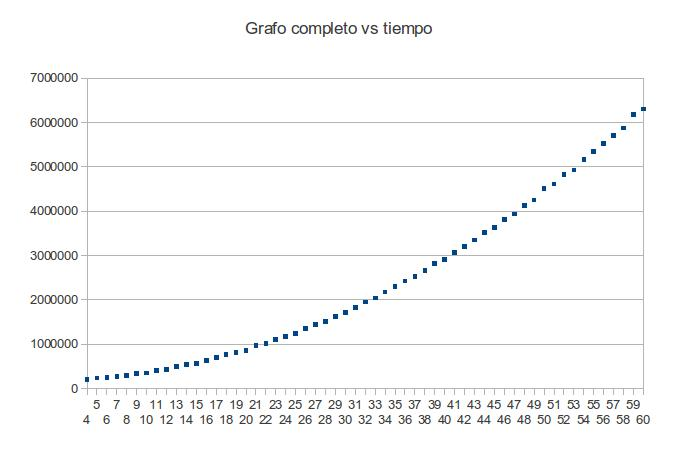
\includegraphics[scale=0.5]{Ej3/resultados1.jpg}
	%\caption{Descripcion de la figura}
	\label{nombreparareferenciar}
  \end{center}
\end{figure}

\newpage
Dividimos por una función cuadratica para ver que se obtiene:

\begin{figure}[h!]
  \begin{center}
	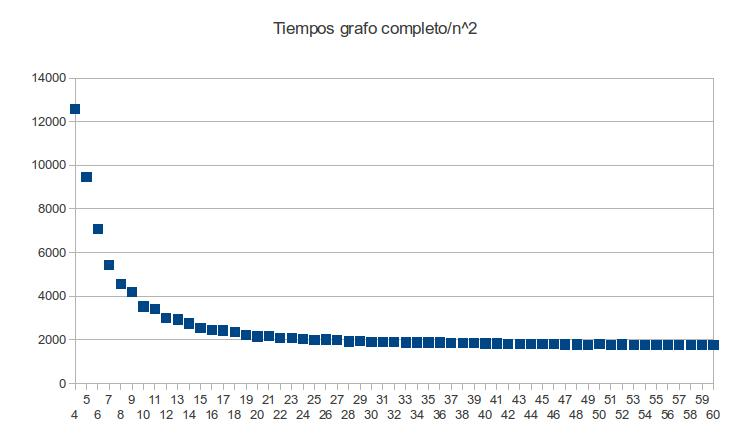
\includegraphics[scale=0.5]{Ej3/resultados2.jpg}
	%\caption{Descripcion de la figura}
	\label{nombreparareferenciar}
  \end{center}
\end{figure}

Si bien en los primeros casos, el algoritmo pareciera no ser lineal, esto puede deverse a que la instancia del problema es muy pequeña y los outliers en ese caso son mayores.
\\
Para las instancias mas grandes se vé que el algoritmo el casi perfectamente constante. Luego, de manera empirica, podemos concluír que nuestro algoritmo es cuadratico con respecto a $n$ en el peor caso.